\documentclass{article}
\usepackage{graphicx} % Required for inserting images
\usepackage{amsmath} 
\usepackage{listings}
\usepackage{xcolor}
\usepackage{float}

\lstset{ 
  language=Python,                % El lenguaje del código
  basicstyle=\ttfamily\footnotesize, % Estilo básico del texto
  keywordstyle=\color{blue},    % Color para palabras clave
  commentstyle=\color{green},   % Color para comentarios
  stringstyle=\color{red},      % Color para strings
  numbers=left,                 % Números de línea a la izquierda
  numberstyle=\tiny\color{gray},% Estilo de los números de línea
  stepnumber=1,                 % Números de línea en cada línea
  numbersep=5pt,                % Separación entre números de línea y código
  backgroundcolor=\color{white},% Color de fondo
  showspaces=false,             % No mostrar espacios
  showstringspaces=false,       % No mostrar espacios en strings
  showtabs=false,               % No mostrar tabs
  frame=single,                 % Cuadro alrededor del código
  tabsize=2,                    % Tamaño de tabulación
  captionpos=b,                 % Título debajo del código
  breaklines=true,              % Cortar líneas largas
  breakatwhitespace=false,      % Cortar solo en espacios
  escapeinside={\%*}{*)}        % Añadir LaTeX dentro del código
}

\title{Nivel 3 Introduccion a Programacion}
\author{Tomas Rodriguez - 202212868}
\date{Abril 2022}

\begin{document}
\maketitle
\section{Intrucciones Iterativas - While}
Las instrucciones iterativas son aquellas las cuales se necesitan repetir u determinado numero de veces o hasta que se cumpla una condicion. 
\subsection{While}
\begin{lstlisting}[language=Python, caption=Ciclo While]
While condicion: 
    accion
    ...
    accion 
    accion
\end{lstlisting}
La instruccion \textbf{While} se determina por la condicion boolena presente en esta, es decir, mientras se cumpla la \textit{condicion}, las acciones se van a ejecutar. Estas se dejaran de ejecutar una vez la condicion del \textbf{While} no se cumpla.\\
Una caracteristica fundamental de estos ciclos, es que dentro de si mismos se tiene que ir cambiando la variable la cual determina la condicion de ejecucion, de lo contrario, se formara un ciclo \textbf{infinito}.
\begin{lstlisting}[language=Python, caption= While infinito]
i  = 0
while i < 10:
    print(i)
print("Fin")
\end{lstlisting}
como se observa en el anterior codigo, la vaiable \textbf{i} jamas va a cambiar, por ende siempre sera menor a 10 lo que generara un ciclo infinito. La forma correcta de modelar este codigo es cambiando la variable que determina la condicion de la siguente manera:
\begin{lstlisting}[language=Python, caption=While Finito ]
i  = 0
while i < 10:
    print(i)
    i += 1
print("Fin")
\end{lstlisting}
Con este pequeño cambio, la variable podra llegar a 10 y el bucle llegara un momento en el que no se ejecute mas. 
\subsubsection{Los Centinelas}
Los centinelas, son variables las cuales nos permiten controlar las ejecuciones de un ciclo. Normalmente es mas complejo pensar en condiciones de parada de un ciclo que las de continuacion, entonces, los centinelas los cuales normalmente son \textit{Booleanos}, nos permiten simplificar esto:
\begin{lstlisting}[language=Python, caption=While Finito ]
def mcd(n1,n2):
n = min(n1,n2)
encontrado = False
while encontrado == False:
    if (n1%n == 0 and n2%n == 0):
        encontrado = True
    else:
        n -= 1
return n
\end{lstlisting}
Lo que hace el codigo anterior es encontrar el MCD entre dos numeros, se sabe que el MCD de dos numeros es aquel que cuando se dividen ambos numeros entre otro y el residuo de ambos es 0, entonces ese es el MCD, por ende, es mas facil pensar en esa condicion que utilizar leyes de morgan (Nivel 2) para cambiar la expresion booleana. 
\section{Cadenas de caracteres o Strings 2}
Aparte de lo visto en el modulo 2 del curso, hay algunas caracteristicas adicionales sobre los \textbf{strings} las cuales se deben conocer.
\subsection{Indexaciones}
Esto consiste en la capacidad de acceder a un elemento especifico de una cadena, ejemplo: 
\begin{lstlisting}[language=Python, caption=Indexacion String]
string = "Hola Mundo"
print(string[1])
\end{lstlisting}
El resultado del codigo anterior va a ser "o", ya que en programacion, todos los elementos que son iterables, es decir que se pueden recorrer con ciclos, inician desde el indice 0, por esto mismo, el ultimo elemento de la cadena no es: 
\begin{lstlisting}[language=Python, caption=Indexacion String 2 ]
string[len(string)]
\end{lstlisting}
si no sera:
\begin{lstlisting}[language=Python, caption=Indexacion String 3 ]
string[len(string)-1]
\end{lstlisting}
Si se interara usar la forma de acceder sin el \(-1\) entonces python hara raise de un error llamado \textbf{IndexError}.\\
Otra forma de buscar caracteres en un string es con el metodo \textbf{find}. Este metodo recibe una cadena y nos indica la posicion en la que esta se encuentra, sin embargo, si no encuentra la cadena, devuelve \(-1\).
\begin{lstlisting}[language=Python, caption=Metodo Find]
string = 'Hola'
string.find('H')
\end{lstlisting}
\subsection{Sub-Cadenas}
Las subcadenas son partes de una cadena principal, es decir son recortes o partes mas pequeñas de la cadena original. Para obtener subcadenas se hacer por medio del operador de \textbf{slicing} el cual consiste en cortar un string.
\begin{lstlisting}[language=Python, caption=Slicing String 1 ]
x = 'Piratas'
s = x[n:m]
\end{lstlisting}
n y m son numeros que indican n el indice de inicio y hasta donde se recorta m-1 caracteres. Si se omite alguno de los numeros de inicio o fin es decir que la subcadena va desde el inicio o va hasta el final.
\begin{lstlisting}[language=Python, caption=Slicing String 2 ]
x = 'Piratas'
s = x[n:]
z = x[:m]
\end{lstlisting}
Ahora bien, existe un tipo de \textbf{slicing} mas avanzado y es implementando pasos. Estos slices se ven de la siguente manera:
\begin{lstlisting}[language=Python, caption=Slicing String 3 ]
x = 'Piratas'
s = x[n:m:a]
\end{lstlisting}
En este se usa un nuevo valor \textbf{a} el cual indica que tantos caracteres se tienen que omitir, se ilustra mejor a continuacion:
\begin{lstlisting}[language=Python, caption=Slicing String 4 ]
x = 'Piratas'
s = x[::2]
print(s)
\end{lstlisting}
El resultado de este codigo sera: \textbf{Prts}\\
Ahora bien, cabe resaltar que las cadenas son \textbf{inmutables}, es decir, no se pueden cambiar los valores de una posicion ya definida, para ello se tiene que usar slicing para crear 2 subcadenas y poner el nuevo caracter en medio:
\begin{lstlisting}[language=Python, caption=Inmutabilidad]
x = 'Hola mi jente'
correccion = x[:8] + 'g' + x[9:]
\end{lstlisting}
El resultado de este codigo sera: Hola mi gente
\section{Instrucciones Iterativas - For}
Asi como la instruccion While, el \textbf{For} es una instruccion iterativa, se podria decir que este tiene 2 tipos distintos
\begin{itemize}
    \item in range: Funciona como el While con los indices de los elementos
    \item in: funciona recorriendo ya no los indices sino aquellos elementos que componen uno mas grande.
\end{itemize}
\begin{lstlisting}[language=Python, caption=For in range]
x = 'Hola mi jente'
for i in range(len(x)):
    print(x[i])
\end{lstlisting}
\begin{lstlisting}[language=Python, caption=For each]
x = 'Hola mi jente'
for caracter in x:
    print(caracter)
\end{lstlisting}
Estos dos son equivalentes, solo que uno es con indices y el otro con los sub-elementos que conforman a uno mas grande. Ahora bien, en el caso del \textbf{For in range}, la funcion \textbf{range()} puede recibir 3 parametros al igual que los slices: 
\begin{itemize}
    \item Primer Parametro: Indice de inicio
    \item Segundo Parametro: Indice de Fin
    \item Tercer Parametro: Saltos de indices
\end{itemize}
\section{Listas}
Las listas son colecciones de valores y en python es una estructura de datos. Aquellos elementos que conforman una lista son llamados elementos o items, cabe resaltar que en \textbf{python} las listas pueden albergar cualquier tipo de dato. \\
Las listas son muy similiares a los string, ya que al fin al cabo son secuencias de elementos o caracteres (caso String), pero, ademas estos comparten muchas operaciones ya conocidas:
\begin{enumerate}
    \item Pueden ser parametros de funciones
    \item Se puede usar la funcion \textit{len()} para conocer la cantidad de elementos en la lista
    \item El operador de suma \(+\) se puede usar para concatenar dos listas distintas
    \item Se pueden indexar los elementos de la lista
    \item Se puede usar el operador de corte o slicing 
    \item Se puede usar las instrucciones iterativas sobre estas
    \item Funciones \textit{max() y min()} funcionan en listas
\end{enumerate}
Ahora bien, las listas tienen diversas formas de iniciarse o declararse, algunas de estas son:
\begin{lstlisting}[language=Python, caption= Declaracion de una lista]
a = []
\end{lstlisting}
\begin{lstlisting}[language=Python, caption= Combinacion de List y Range para generar una lista]
a = list(range(1,4))
\end{lstlisting}
Este codigo va a generar el siguente array:
\[[
\begin{array}{ccc}
    1 & 2 & 3
\end{array}
]
\]
\begin{lstlisting}[language=Python, caption= Operador de multiplicacion para generar una lista]
a = [0]*10
\end{lstlisting}
Este codigo va a generar el siguente array:
\[[
\begin{array}{cccccccccc}
    0 & 0 & 0 & 0 & 0 & 0 & 0 & 0 & 0 & 0 
\end{array}
]
\]
\subsection{Operaciones de Listas}
Asi como en las cadenas, las listas tienen operaciones muy parecidas a aquellas que se realizan sobre las cadenas de caracteres, algunas de estas son:
\begin{lstlisting}[language=Python, caption= Comparacion de Listas]
if lista1 == lista2:
\end{lstlisting}
La comparacion del operador \( == \) en listas funciona de la siguente forma:
\begin{itemize}
    \item Primero compara el tamaño de cada lista, si este es diferente devuelve False.
    \item Si pasa el primer filtro, despues compara elemento por elemento de izquierda a derecha, si un solo elemento es diferente devuelve False.
\end{itemize}
Ahora bien, estas dos reglas se cumplen para todas las operaciones de comparacion como \( < ,\ <= ,\ > ,\ >=\) con sus repesectivas definiciones claro esta solo que en orden inverso, primero se revisan los elementos y despues el tamaño de la lista.\\
\begin{lstlisting}[language=Python, caption= Modificaciones en Listas]
lista1[0] = 1
lista1[1:3] = [2,3]
\end{lstlisting}
Para modificar elementos que estan dentro de una lista se usa la operacion de \textbf{indexacion} con el fin de alterar o modificar el valor que se encuentra en dicha posicion o incluso se puede usar la operacion de \textbf{slicing} para llevar a cabo estas modificaciones.
\begin{lstlisting}[language=Python, caption= Eliminacion de elementos de Listas]
del lista1[0]
del lista1[1:3]
\end{lstlisting}
Ahora bien, para las operaciones de eliminacion se usa la palabra reservada de \textbf{del} la cual indica delete, esta se puede combinar con las operaciones de modificacion de listas antes vistas.\\
\begin{lstlisting}[language=Python, caption= Clonacion de Listas]
a = [1,2,3]
b = a[:]
\end{lstlisting}
Esta operacion se conoce como clonacion de listas, es decir, se va a hacer una copia de la lista de la variable \(a\) en la variable \(b\). 
\subsubsection{Operador is}
\begin{lstlisting}[language=Python, caption= Eliminacion de elementos de Listas]
a = [1,2,3]
b = [1,2,3]
c = a
\end{lstlisting}
En este codigo si se hace un codigo de evaluacion para ver si las listas \(a,b,c\) son iguales, el resultado va a ser \(True\) ya que todas las variables tienen como valor \([1,2,3]\), sin embargo, si usamos este nuevo operador \(is\) tenemos como resultado lo siguente:
\begin{lstlisting}[language=Python, caption= Operador is en Listas]
a is b
b is c
a is c
\end{lstlisting}
El resultado de evaluar dichas condiciones es:
\begin{enumerate}
    \item False
    \item False
    \item True
\end{enumerate}
Esto debido a que si nos vamos a observar que pasa en la memoria de nuestro computador en el \(Listing \ 22\) estara pasando lo siguente: 
\begin{figure}[H]
    \centering
    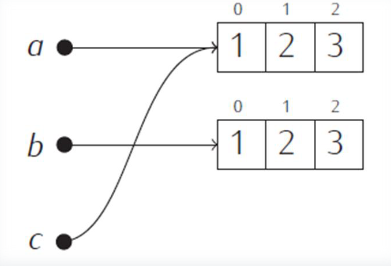
\includegraphics[width=.5\linewidth]{MemoryOperationIs.png}
    \caption{Representacion Memoria}
    \label{fig:enter-label}
\end{figure}
Esto nos indica que, tecnicamente las variables \(a\) y \(c\) tienen un unico valor compartido, sin embargo, \(b\) tiene un unico valor para si mismo, por ello, al usar la operacion \(is\) tan solo la expresion \(a \ is \ c\) da como resultado \(True\).\\
Ahora bien, en el caso de la operacion de \textbf{clonacion}, la lista clonada en la otra variable no va a estar referenciada al mismo lugar en memoria si no que cada lista tendra su lugar en memoria distinto.
\subsection{Metodos de Listas}
Asi como las listas poseen operaciones, estas tambien poseen unos metodos los cuales se escriben de la siguente manera:
\begin{lstlisting}[language=Python, caption= Metodos de Listas]
lista.metodo(parametros)
\end{lstlisting}
Los metodos son funciones que hacen parte de las listas, es decir, estas tambien pueden tener parametros, retornos, etc. algunos de los mas importantes son:
\begin{itemize}
    \item append(elemento): Adiciona un elemento al final de la lista
    \item insert(i,elemento): Adiciona un elemento en la posicion i de la lista
    \item count(elemento): Cuenta cuantas veces se repite un elemento en la lista
    \item extend(listaNueva): Junta dos listas, aquella a la cual se le aplica el metodo y la que se pasa por parametro, para que aquella que es parametro se agregren sus elementos al final de la lista que invoca el metodo
    \item index(elemento): Devuelve el indice de la primera ocurrencia en donde se encuentra el elemento.
    \item reverse(): Le da la vuelta a todos los elementos, es decir, invierte el orden de la lista
    \item sort(): ordena los elementos en la lista
    \item remove(elemento): elimina la primera ocurrencia del elemento en la lista
    \item copy(): Hace una copia de la lista
    \item pop(indice): Dado un indice, elimina el elemento que pertenece a dicho indice y lo devuelve
    \item clear(): Elimina todos los elementos de una lista
\end{itemize}
\subsection{De cadenas a listas y viceversa}
Ahora bien, despues de conocer las operaciones y metodos de las listas, hay un uso adicional que estas tienen y es la capacidad de separar y hacer strings a partir de sus elementos.
\begin{lstlisting}[language=Python, caption= Metodo Split de cadena a lista]
cadena = "uno dos tres"
lista = cadena.split(" ")
\end{lstlisting}
En este codigo se usa el metodo \(split\) de las cadenas de caracteres para separar la cadena en una lista que da como resultado: \([uno,dos,tres]\), esto fue posible gracias a que en la cadena, las palabras estaban separadas por espacion en blanco, por ende, el parametro que usa el metodo \(split\) es el separador de la cadena, es decir, porque estan separadas las palabras o elementos.
\begin{lstlisting}[language=Python, caption= Metodo Join de Lista a cadena]
cadenaReconstruida = " ".join(lista)
\end{lstlisting}
Ahora bien, el metodo inverso a \(split\) es el metodo \(join\), el cual como indica su nombre es juntar los elementos de la lista en un unico string.
\section{Recorridos en listas y diccionarios}
Los recorridos para estas dos estructuras de datos son similares pero a la vez diferentes por la naturaleza de cada uno.
\subsection{Recorridos en listas}
\subsubsection{Recorridos Totales}
Este tipo de recorridos se llevan a cabo con instrucciones \textbf{While}, \textbf{For in range} y \textbf{For each}. Estos recorridos son aquellos en los cuales se va recorriendo los indices o elementos de una lista uno por uno hasta el final de la lista.
\subsubsection{Recorridos Parciales}
Este tipo de recorridos son lo contrario a los totales, en estos, se busca que la cantidad a elementos a recorrer sea lo minimo hasta cumplir cierto objetivo, es decir, su funcion es que se cumpla una condicion con el fin de darles parada y que no se lleven hasta el final de la lista. Los unicos recorridos capaces de lograr esto son el \textbf{While} y el \textbf{While con centinela}, algunos ejemplos son:
\begin{lstlisting}[language=Python, caption= While con centinela]
def posicion_recorrido_parcial_con_centinela(lista: list, buscado: int) -> int:
    i = 0
    posicion = -1
    ya_encontre = False
    while i < len(lista) and ya_encontre == False:
        if lista[i] == buscado:
            ya_encontre = True
            posicion = i
        i += 1
    return posicion
\end{lstlisting}
\begin{lstlisting}[language=Python, caption= While sin centinela]
def posicion_recorrido_parcial_sin_centinela(lista: list, buscado: int) -> int:
    i = 0
    while i < len(lista) and lista[i] != buscado:
        i += 1
    if i == len(lista):
        posicion = -1
    else:
        posicion = i
    return posicion
\end{lstlisting}
\subsection{Recorridos en diccionarios}
En el caso de los diccionarios existen tambien 2 tipos de recorridos, aquellos que son llave y aquellos que son por valor, sin embargo, estos recorridos usan los mismos tipos de recorridos que las listas, ya que para recorrer los diccionarios por llaves se usa el metodo \(keys()\) para que se recorra una lista de las llaves del diccionario, o si es por valor, se usa el metodo \(values()\) que tambien devuelve una lista con los valores para ser recorridos.
\section{Manejo de archivos}
Los archivos son objetos donde podemos llevar a cabo operaciones de lectura y escritura de informacion. En programacion, para usar dichos objetos se deben llevar a cabo 3 pasos:
\begin{enumerate}
    \item Abrir el archivo: funcion \(open(nombreArchivo, \ accion)\), donde la accion puede ser: "r" de read, "w" de write o "a" de adicion
    \item Leer o escribir la informacion: Dependiendo la accion en la funcion \(open\) se usa \(readline\) o \(write\)
    \item Cerrar el archivo: Se realiza con la funcion \(close\)
\end{enumerate}
\end{document}

